\documentclass[12pt,landscape,letterpaper]{article}
%Preamble:
\input{sl_graphics_preamble.tex}
\graphicspath{{"Figures/"}}
\usepackage[margin=1in]{geometry}
\usepackage{array}
\setlength{\extrarowheight}{0.5cm}

\begin{document}
\pagestyle{empty}

\begin{flushleft}
\begin{tabular}{>{\sffamily\bfseries}rc!{\hspace{0.5cm}}c!{\hspace{0.5cm}}c}
  % after \\: \hline or \cline{col1-col2} \cline{col3-col4} ...
  a & \aligntop{
\includegraphics[height=2cm]{binary.svg}} & \aligntop{\includegraphics[height=2.4cm]{pooled.svg}} & \aligntop{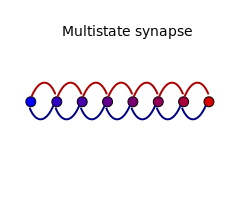
\includegraphics[height=2cm]{multistate.svg}} \\
  b & \aligntop{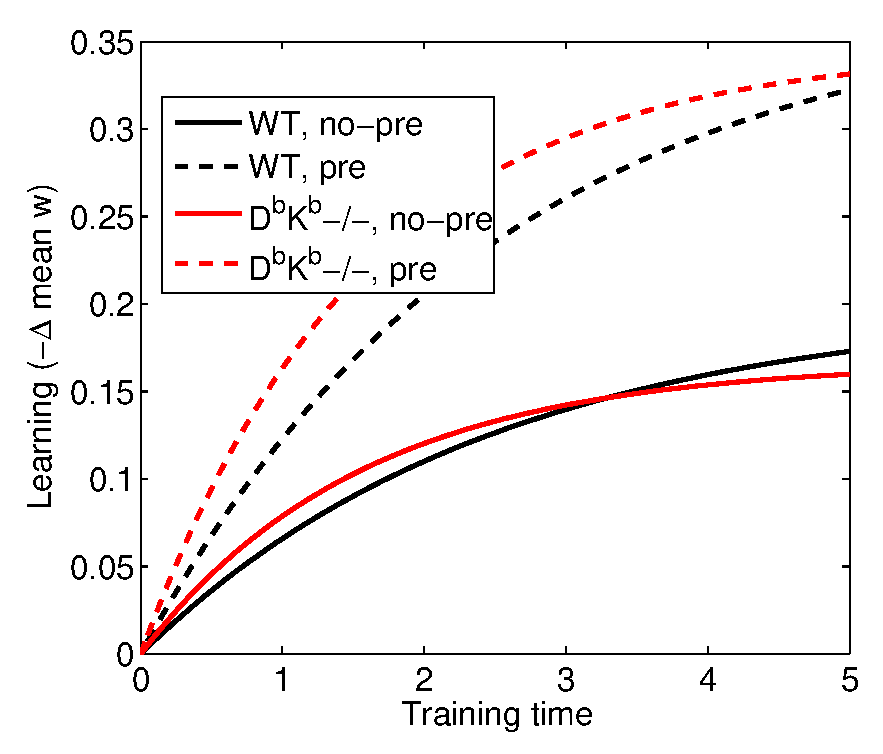
\includegraphics[height=6cm]{binary_learnS.eps}} & \aligntop{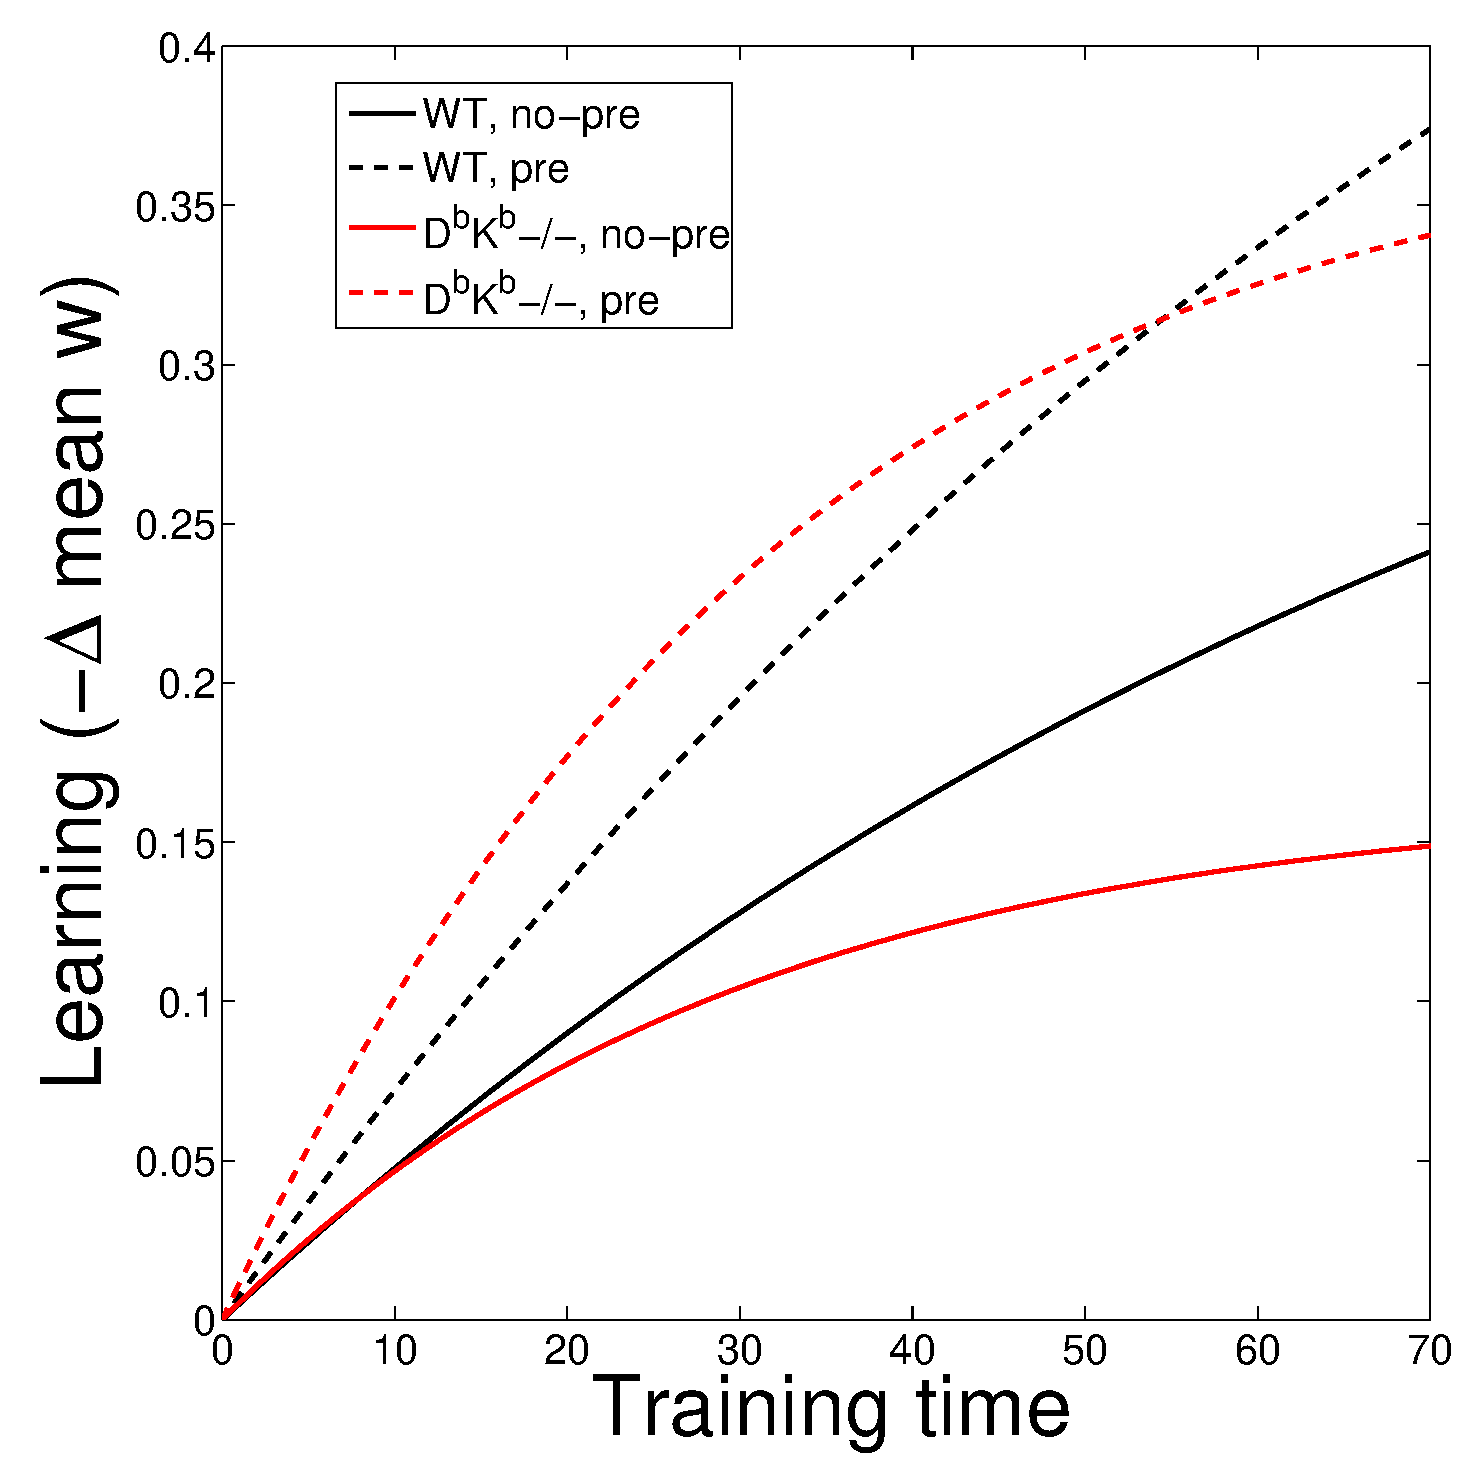
\includegraphics[height=6cm]{pooled_scarce_learnS.eps}} & \aligntop{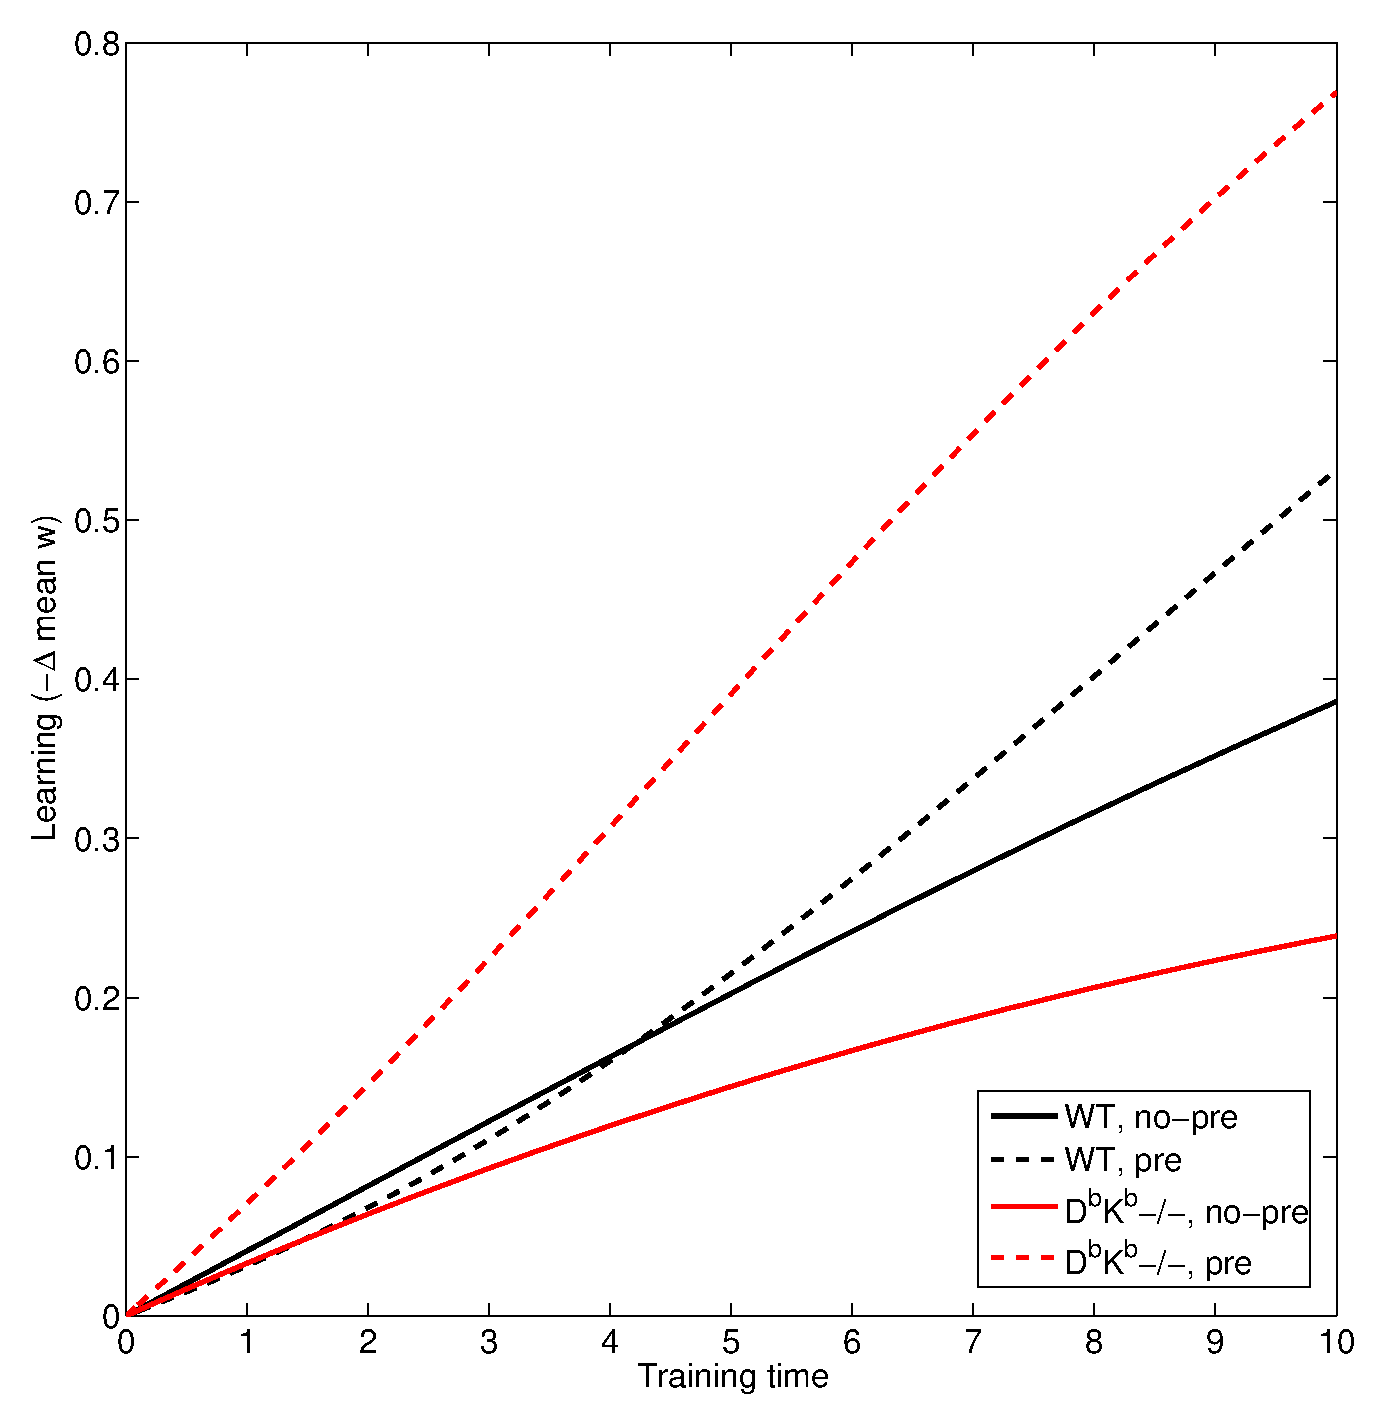
\includegraphics[height=6cm]{multistate_med_learnS.eps}} \\
\end{tabular}
\end{flushleft}




\end{document}
